\chapter{Исследовательская часть}

\section{Среда для тестирования}

Для тестирования разработанного алгоритма применялась облачная платформа Google Colab~\cite{colab}, не требующая установки ПО на локальный компьютер.

% 

\section{Тестирование кластеризации}

Для кластеризации использовались размеченные тексты, разделение которых было известно заранее. Кластеризуемые тексты имели одну из следующих тем: комментаторы, ставки на спорт, спортивная медицина, органическая химия, неорганическая химия, биохимия крови, анамнез.

На рисунках \ref{img:1}-\ref{img:6} приведены графики, показывающие результаты кластеризации методами K-средних и методом C-средних для текстовых данных при заданном количестве кластеров (3, 7 и 10). При визуализации кластеров был использован метод главных компонент (PCA) для уменьшения размерности.

\begin{figure}
	\begin{tabular}[b]{c}
		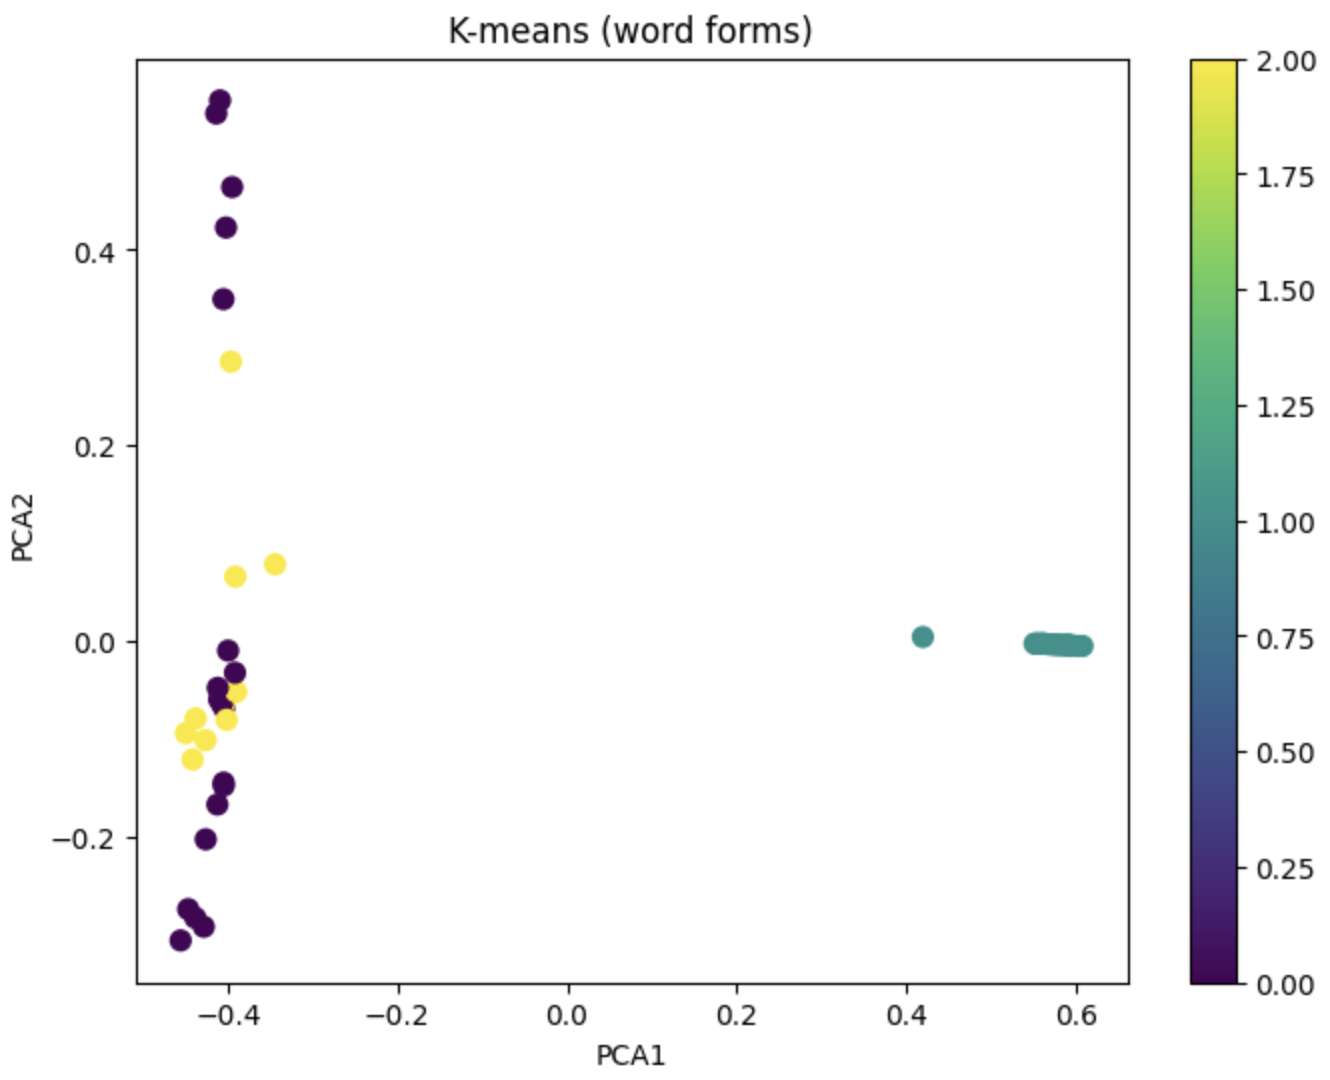
\includegraphics[width=0.475\textwidth]{images/1.png} \\
		\small а) словоформы
	\end{tabular}
	\begin{tabular}[b]{c}
		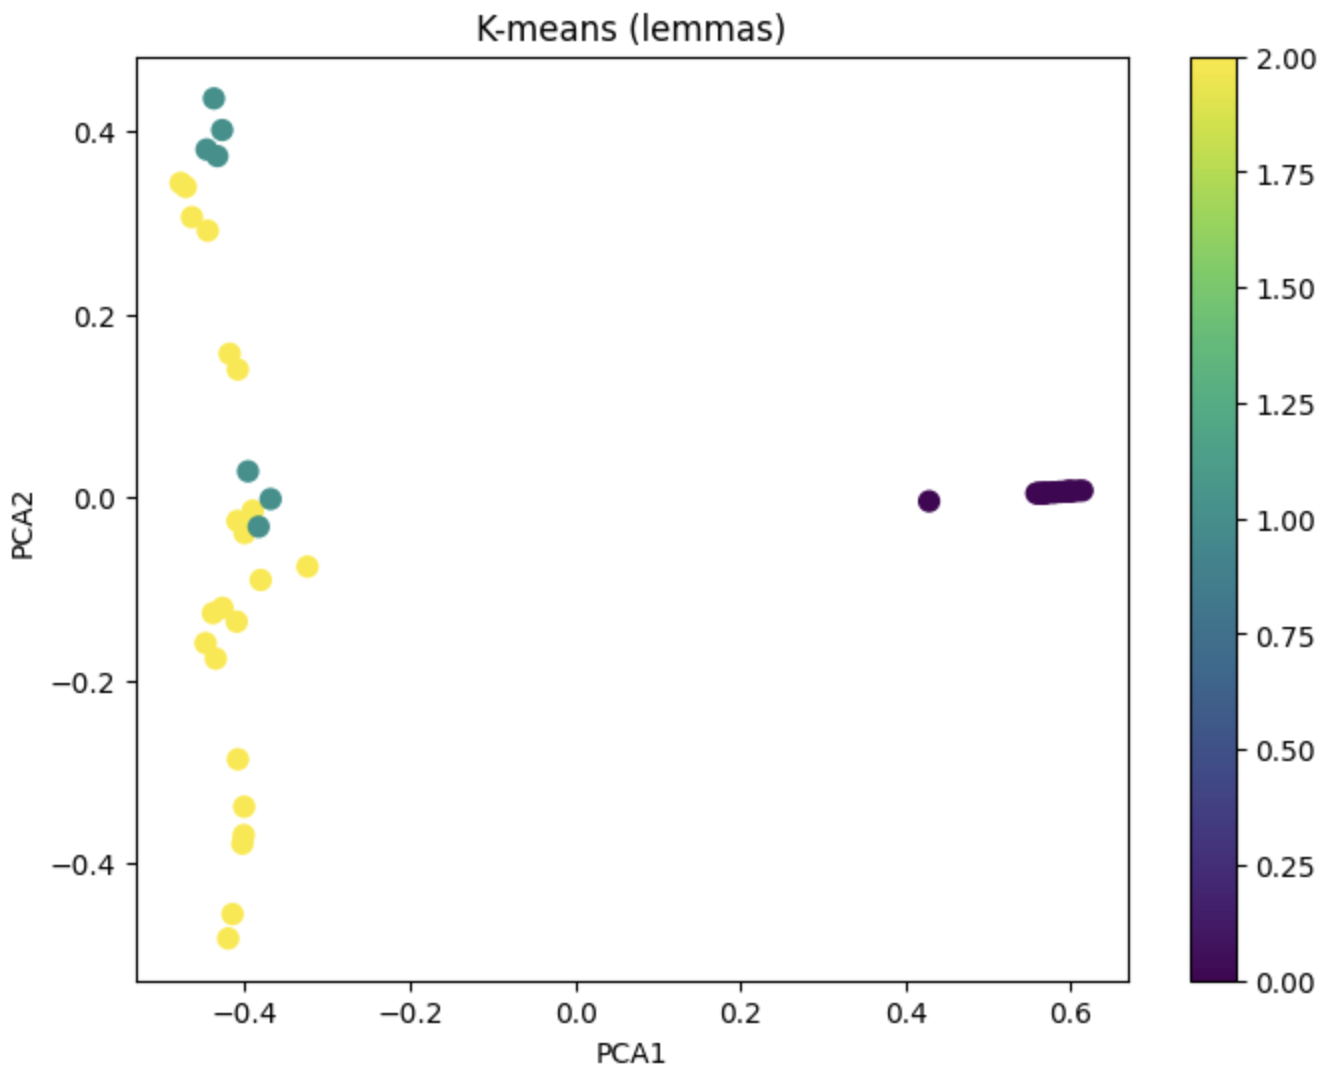
\includegraphics[width=0.475\textwidth]{images/2.png} \\
		\small б) леммы
	\end{tabular}
	\caption{Результаты кластеризации методом K-средних, 3 кластера}
	\label{img:1}
\end{figure}

\begin{figure}
	\begin{tabular}[b]{c}
		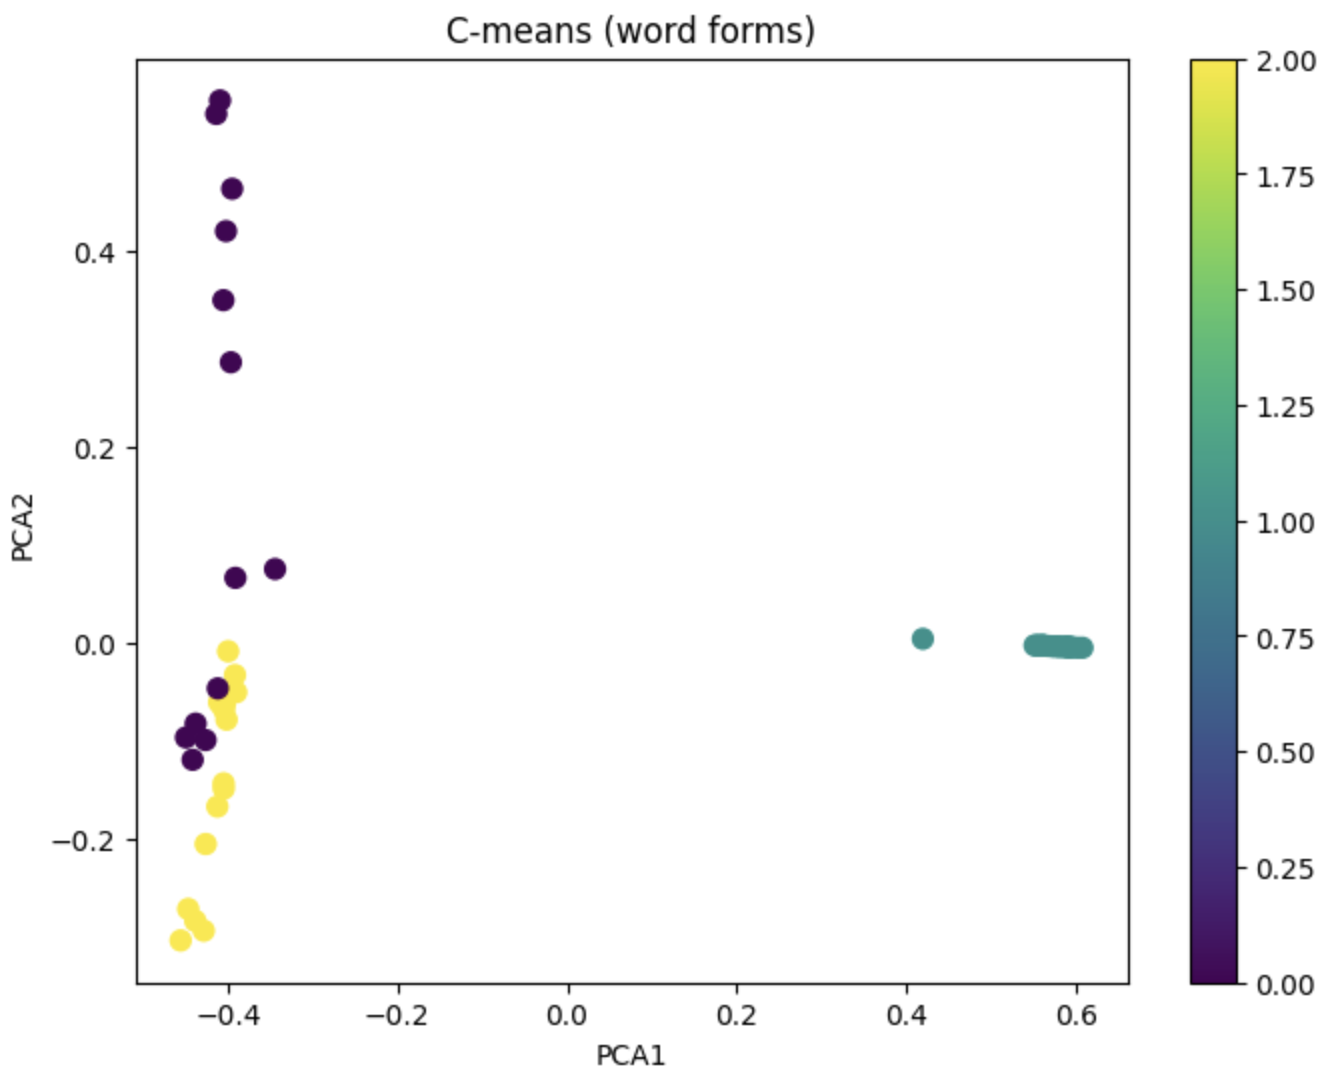
\includegraphics[width=0.475\textwidth]{images/3.png} \\
		\small а) словоформы
	\end{tabular}
	\begin{tabular}[b]{c}
		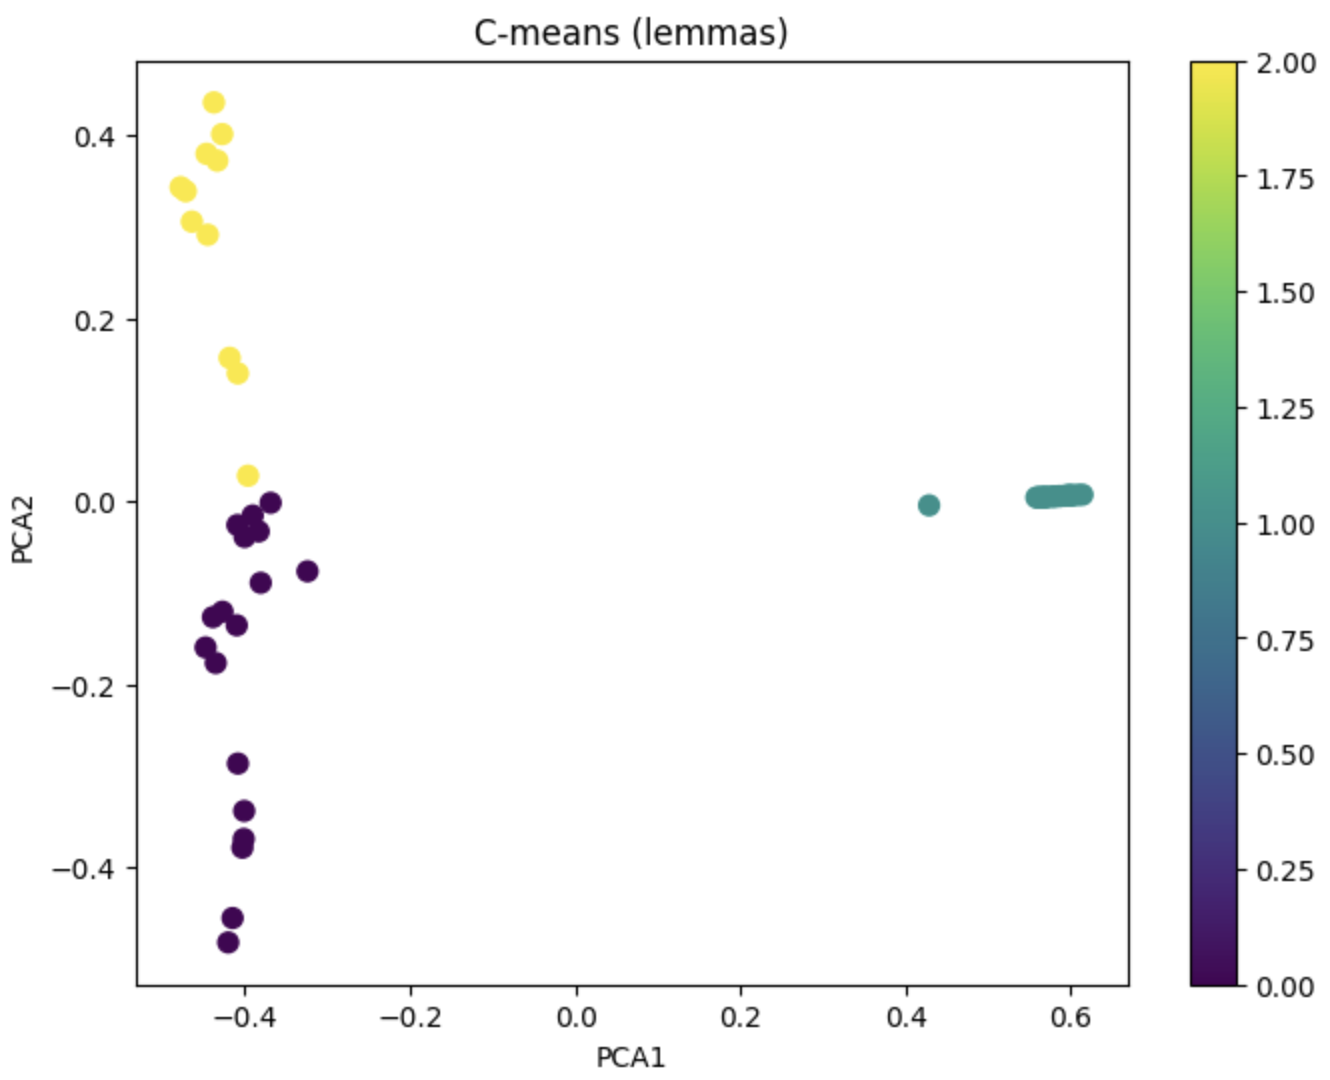
\includegraphics[width=0.475\textwidth]{images/4.png} \\
		\small б) леммы
	\end{tabular}
	\caption{Результаты кластеризации методом C-средних, 3 кластера}
	\label{img:2}
\end{figure}

\begin{figure}
	\begin{tabular}[b]{c}
		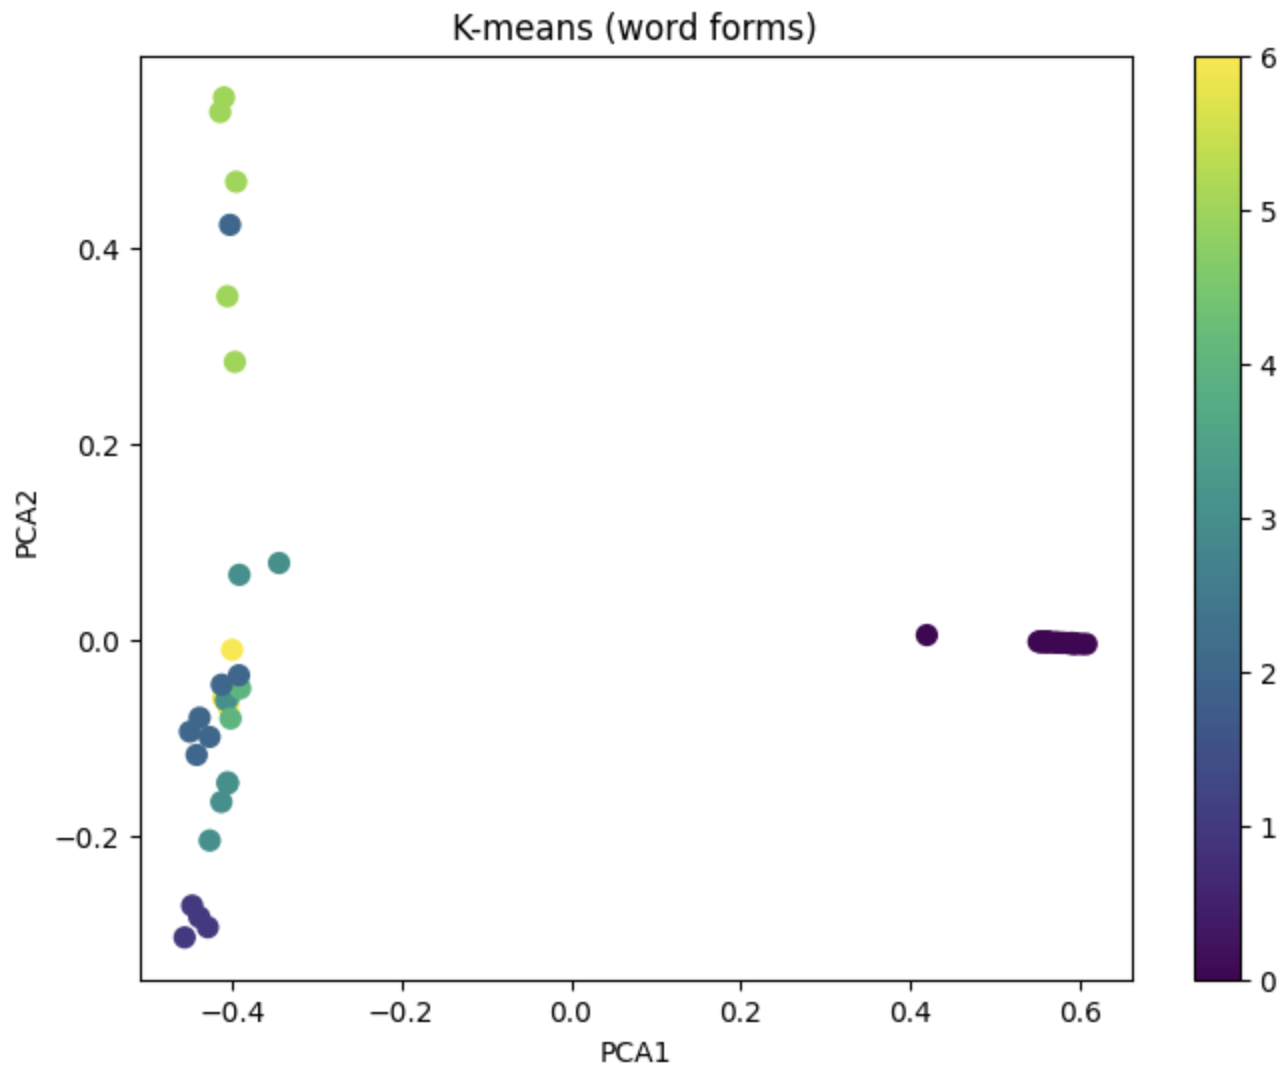
\includegraphics[width=0.475\textwidth]{images/5.png} \\
		\small а) словоформы
	\end{tabular}
	\begin{tabular}[b]{c}
		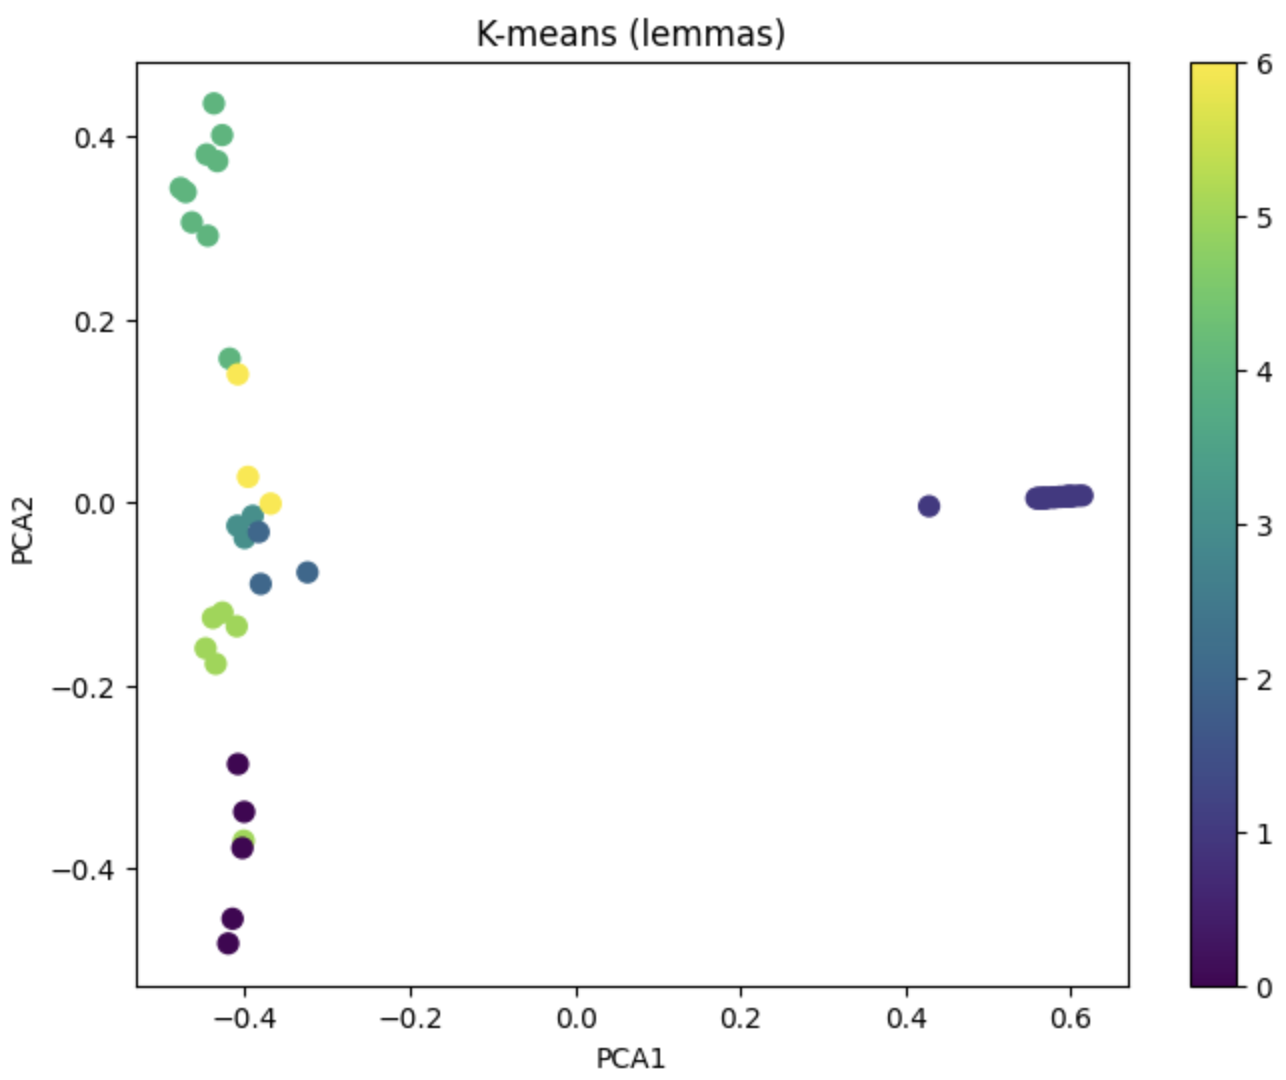
\includegraphics[width=0.475\textwidth]{images/6.png} \\
		\small б) леммы
	\end{tabular}
	\caption{Результаты кластеризации методом K-средних, 7 кластеров}
	\label{img:3}
\end{figure}

\begin{figure}
	\begin{tabular}[b]{c}
		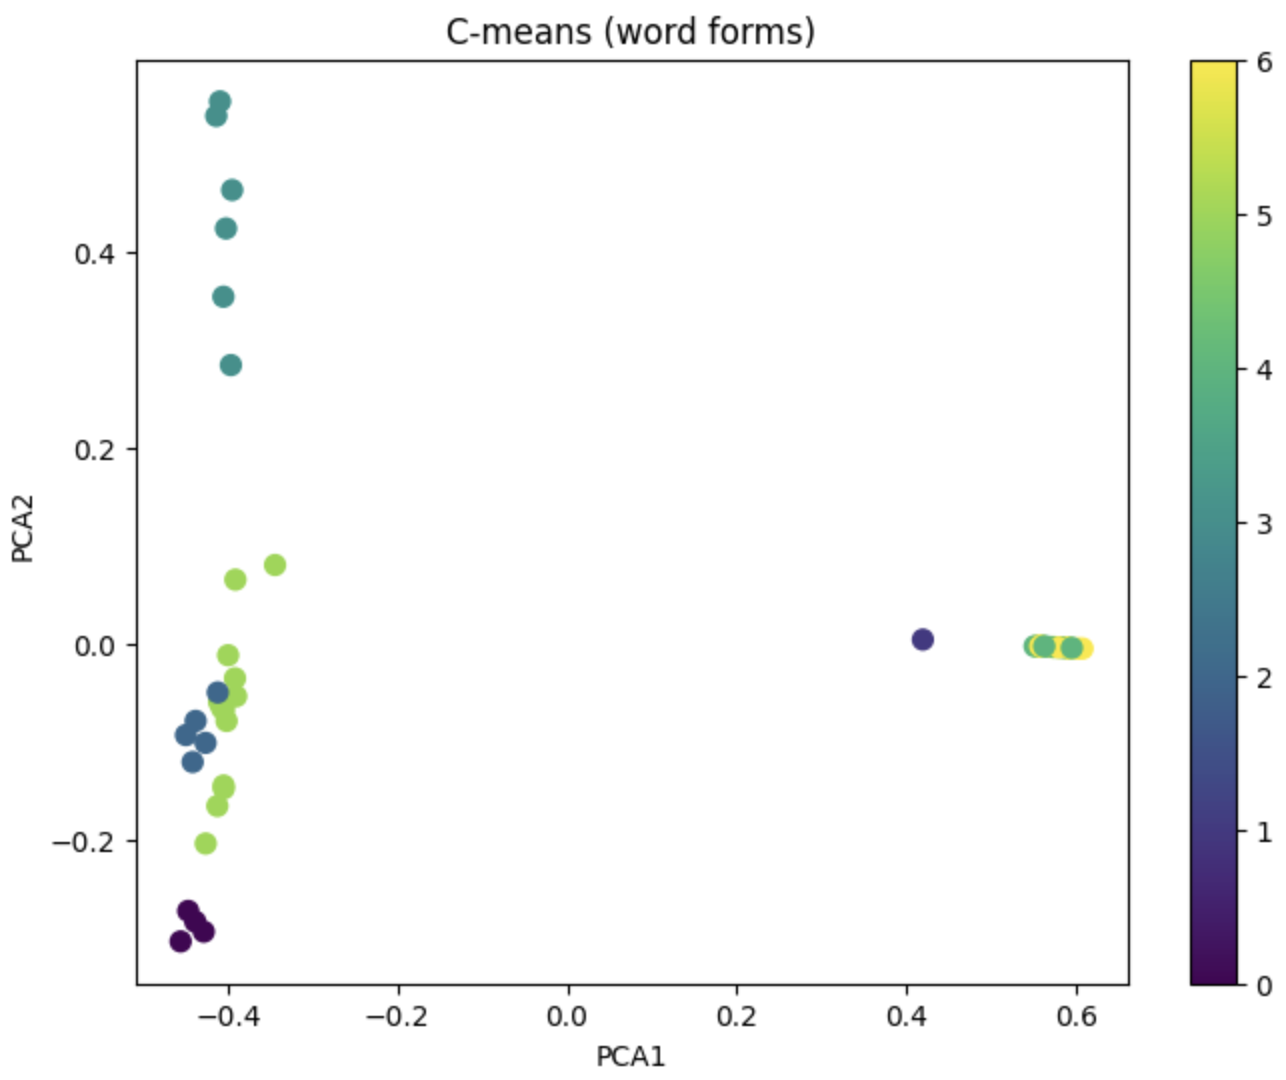
\includegraphics[width=0.475\textwidth]{images/7.png} \\
		\small а) словоформы
	\end{tabular}
	\begin{tabular}[b]{c}
		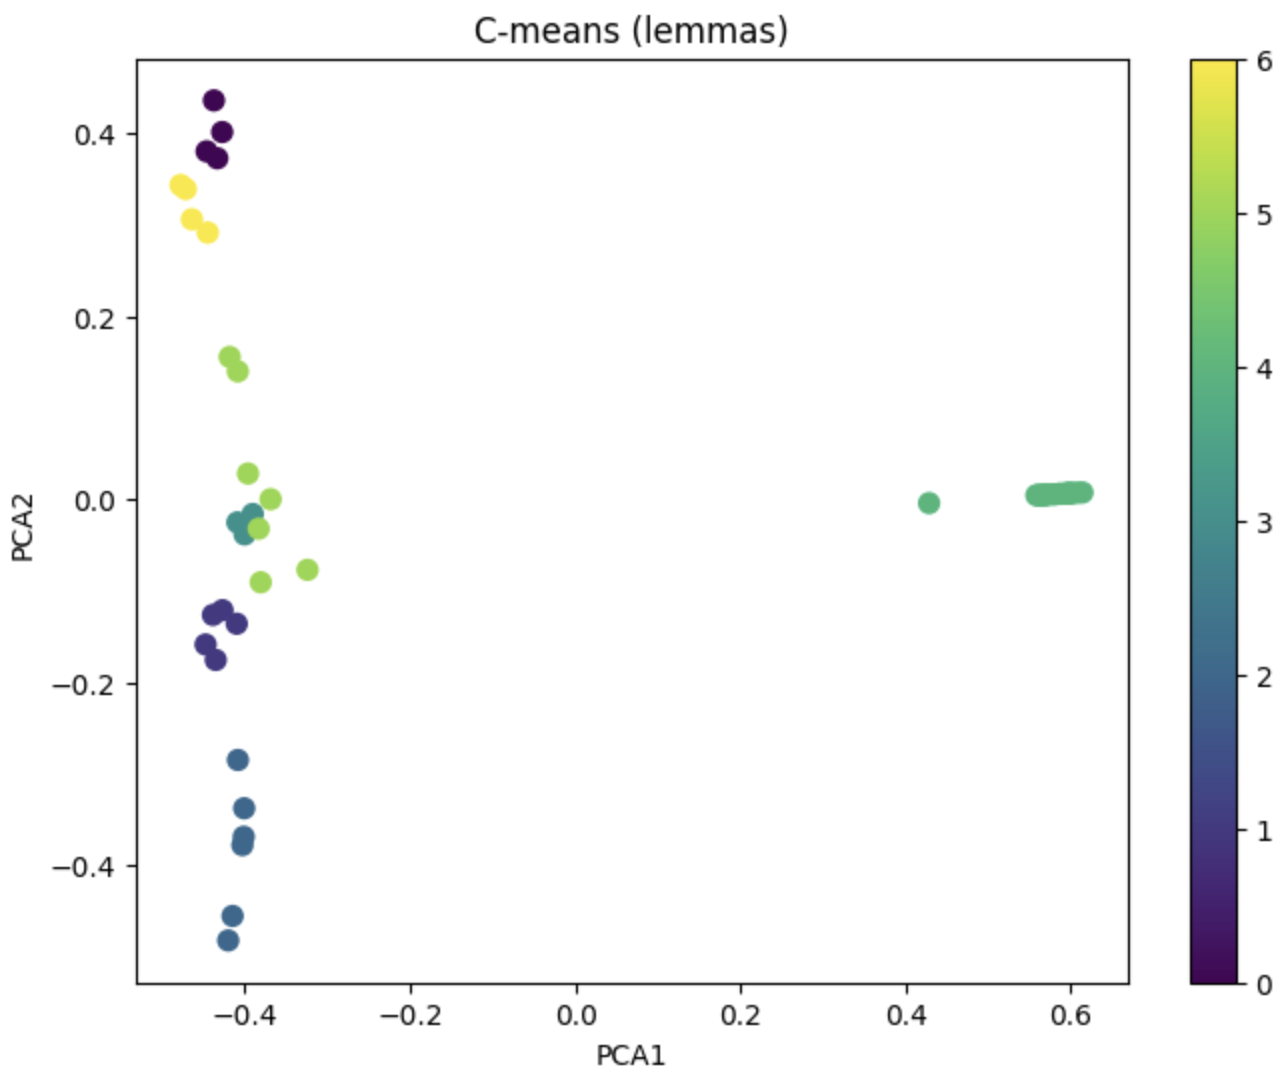
\includegraphics[width=0.475\textwidth]{images/8.png} \\
		\small б) леммы
	\end{tabular}
	\caption{Результаты кластеризации методом C-средних, 7 кластеров}
	\label{img:4}
\end{figure}

\begin{figure}
	\begin{tabular}[b]{c}
		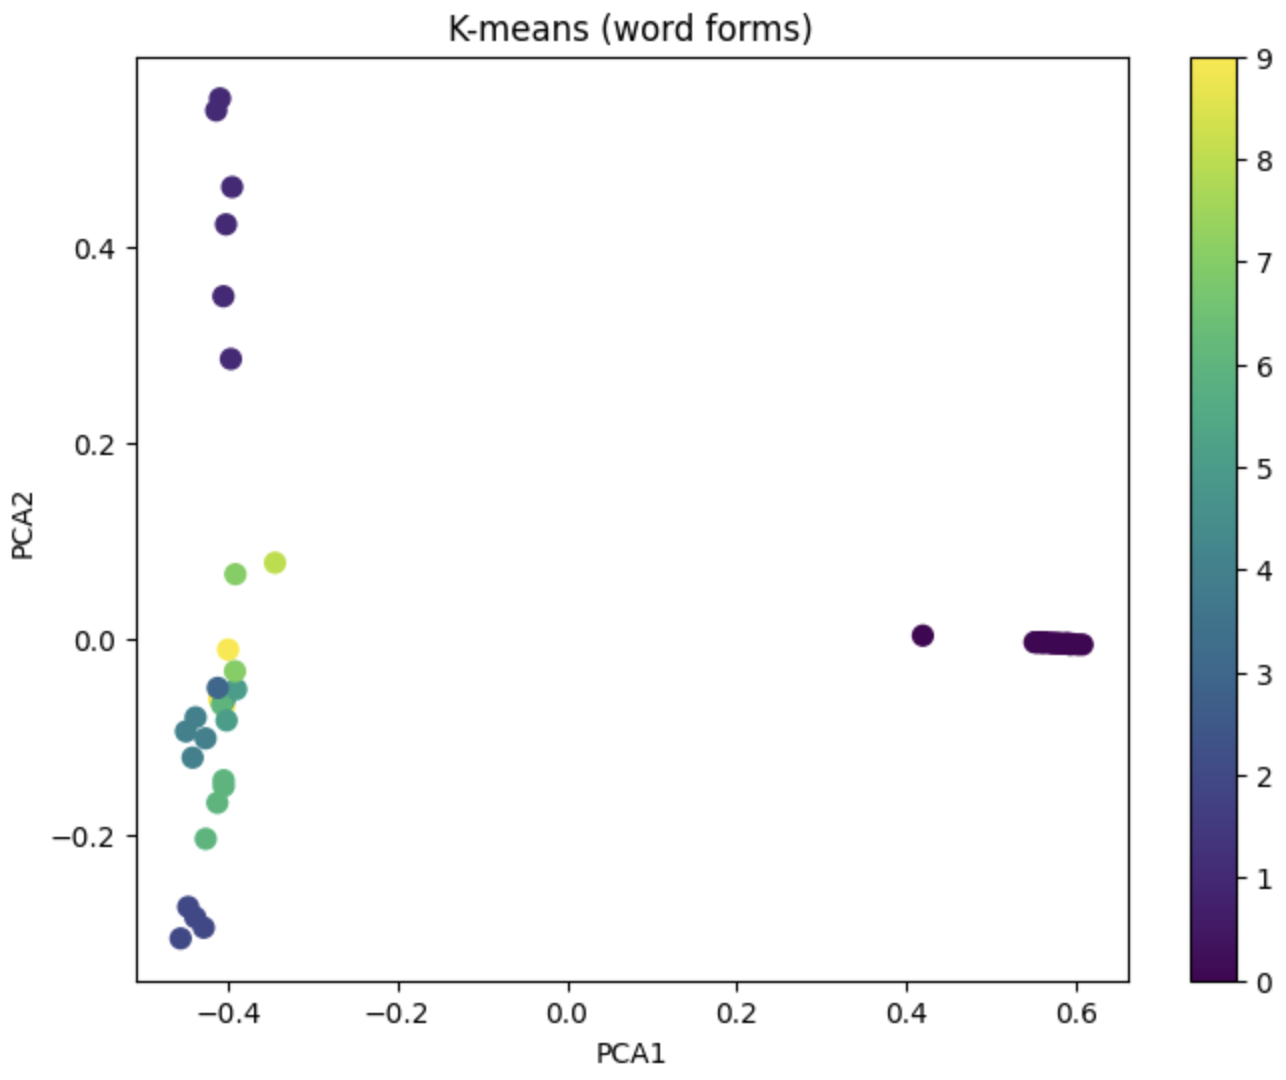
\includegraphics[width=0.475\textwidth]{images/9.png} \\
		\small а) словоформы
	\end{tabular}
	\begin{tabular}[b]{c}
		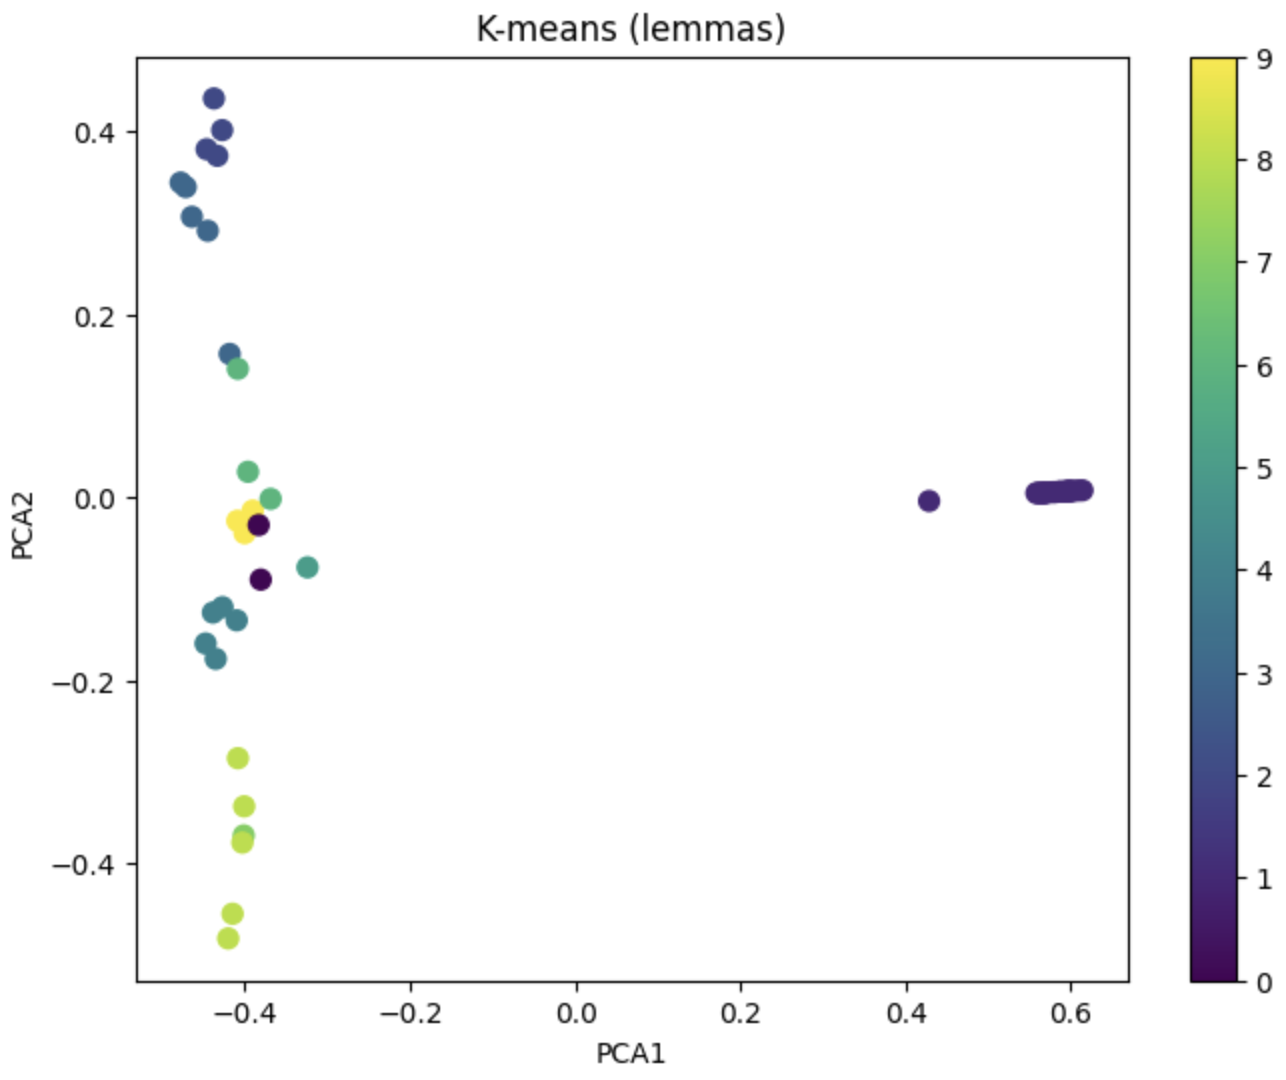
\includegraphics[width=0.475\textwidth]{images/10.png} \\
		\small б) леммы
	\end{tabular}
	\caption{Результаты кластеризации методом K-средних, 10 кластеров}
	\label{img:5}
\end{figure}

\begin{figure}
	\begin{tabular}[b]{c}
		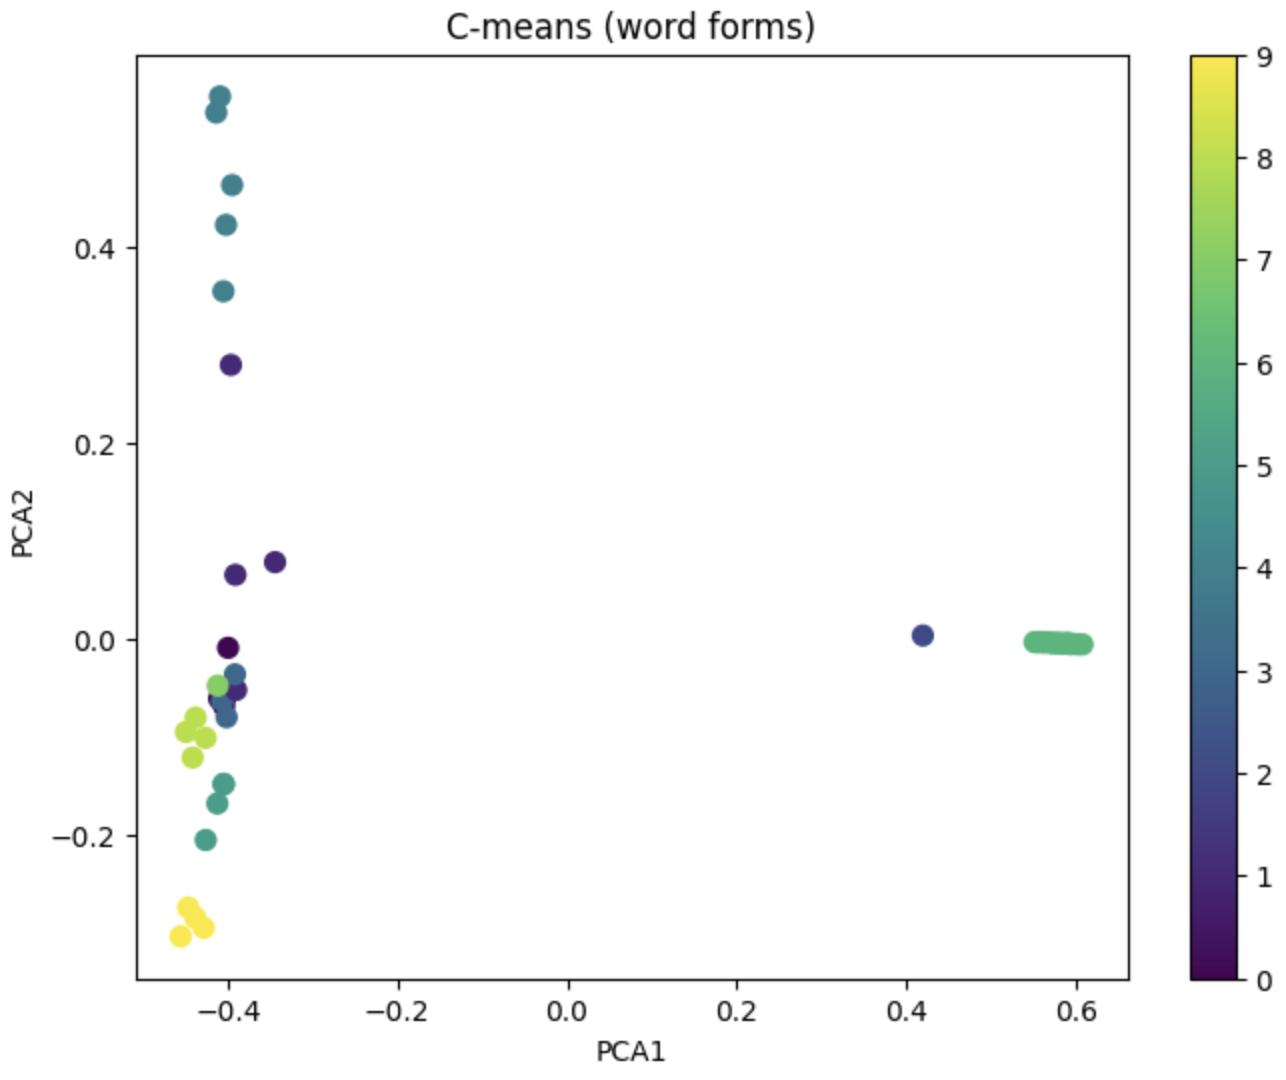
\includegraphics[width=0.475\textwidth]{images/11.png} \\
		\small а) словоформы
	\end{tabular}
	\begin{tabular}[b]{c}
		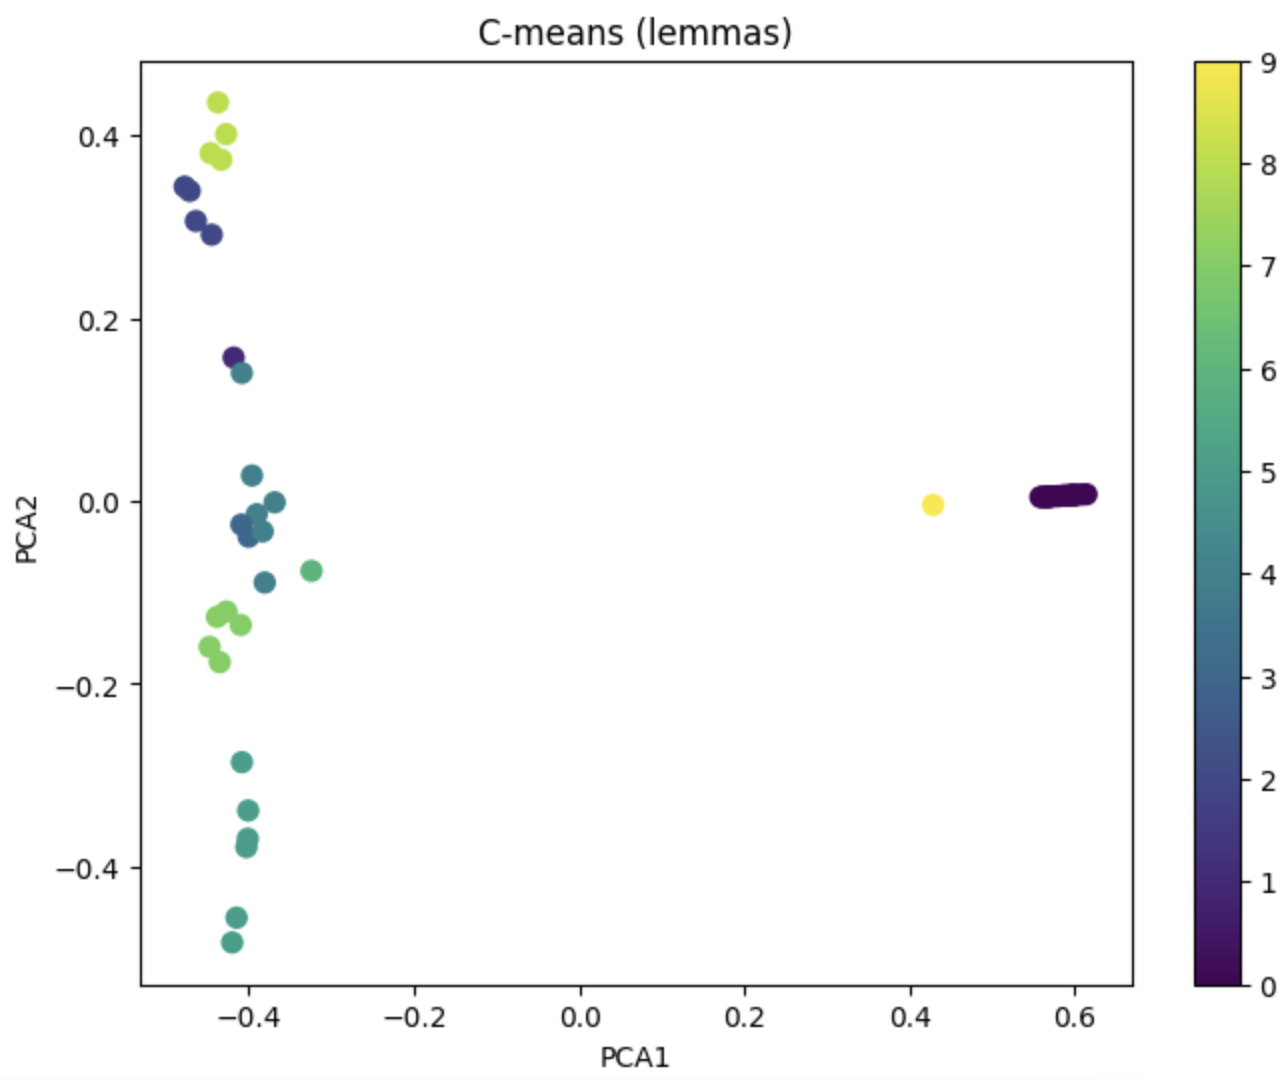
\includegraphics[width=0.475\textwidth]{images/12.png} \\
		\small б) леммы
	\end{tabular}
	\caption{Результаты кластеризации методом C-средних, 10 кластеров}
	\label{img:6}
\end{figure}

\clearpage
\section{Сравнение метрик кластеризации}

\begin{table}[H]
	\centering
	\caption{Сравнение метрик кластеризации для различных подходов}
	\label{tab:prop}
	%\renewcommand{\arraystretch}{1.7}
	\begin{tabular}{|c|c|c|c|c|c|c|}
		\hline
		Метод & \multicolumn{3}{ c| }{Ср. внутрикластерное расст-е} & \multicolumn{3}{ c| }{Ср. межкластерное расст-е} \\ \hline
		Количество кластеров         & ~~~~~~3~~~~~~ & ~~~~~~7~~~~~~ & ~~~~~~10~~~~~~ & ~~~~~~3~~~~~~ & ~~~~~~7~~~~~~ & ~~~~~~10~~~~~~ \\ \hline
		K-средние (словоформы)   & 1.00 & 0.92 & 0.85 & 0.54 & 0.76 & 0.93 \\ \hline
		K-средние (леммы) 			  & 0.96 & 0.89 & 0.82 & 0.57 & 0.78 & 0.95 \\ \hline
		C-средние (словоформы)  & 1.00 & 0.84 & 0.89 & 0.55 & 0.79 & 0.90 \\ \hline
		C-средние (леммы)            & 0.97 & 0.88 & 0.83 & 0.57 & 0.79 &0.98 \\ \hline
	\end{tabular}
\end{table}

\section*{Вывод}

Время выполнения программы в среде Google Colab составило приблизительно 1 минуту. Данный эксперимент был проведён с использованием стандартных вычислительных ресурсов, включая графические ускорители, повышающие производительность обучения.

Качество кластеризации можно оценить как функцию, прямо зависящую от межкластерного расстояния и обратно зависящую от внутрикластерного расстояния. Так, алгоритм K-средних показал наилучшие результаты кластеризации текстовых данных. Лемматизация повышает компактность кластеров и улучшает их разделение, также повышая качество кластеризации. В то же время алгоритм C-средних демонстрирует более размытые границы кластеров, особенно при работе с леммами. Визуализация дополнительно подчёркивает, что выбор метода кластеризации и предварительной обработки текста (лемматизация или её отсутствие) существенно влияет на качество результатов.

\clearpage
